%--- Jens:
\begin{frame}{SUSY theorie}
	\section{SUSY theorie}
	\begin{block}{main ideas}
		\begin{itemize}
\item symmetry under spin transformation\\
\item MSSM: model with fewest new particles% but $10^2$ free parameters\\
\item might solve GUTs and explains dark matter\\
\item quarks \& leptons $\rightarrow$ squarks \& sleptons (spin 0)\\
\item gauge bosons $\rightarrow$ gauginos (spin 1/2) 
		\end{itemize}
	\end{block}

	\begin{figure}[B]
		\centering
	 	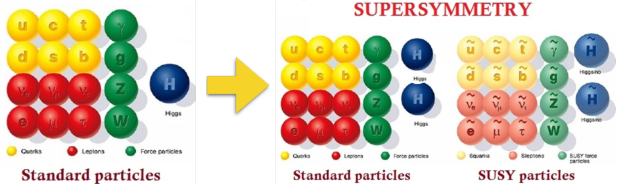
\includegraphics[width=1\textwidth,]{figures/mssm.png}
		\caption{
			\begin{tiny}
	source:  http://inspirehep.net/record/1407182/files/SUSY.png
			\end{tiny}}
	\end{figure}
\end{frame}

%\begin{frame}{LM6 \& LM9}
%\section{LM6 \& LM9}
%\begin{itemize}
%\item benchmark models leads to different branching %ratios \& behaviours\\
%\item LM6 \& LM9 have relative high cross sections\\ 
%\item SUSY-processes: squark \& gluino pair production
%\end{itemize}

%\begin{figure}[H]
%	\centering
%	 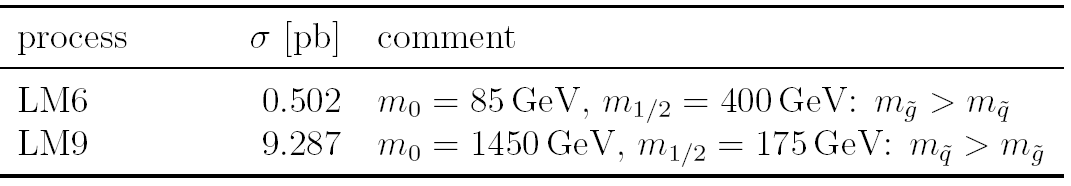
\includegraphics[width=\textwidth,]{figures/properties.png}
	%\caption{aus Übungsblatt Nr. 10}
%\end{figure}

%\end{frame}

\begin{frame}{SUSY im Detektor}
	\section{SUSY im Detektor}
	\begin{block}{manifestation}
		\begin{itemize}
%\item quantum number $R=(-1)^{3B+L+2S} \quad R_{SM}=+1 \qualld R_{SUSY}=-1$ \\
\item conservation of R-parity leads to stable LSP\\
\item LSP is only weak interacting, reconstructable via $\slashed{H}_T$ \\
\item SUSY production: \quad gluino or squark pair production\\
\item SUSY decay: \quad $\tilde{g} \rightarrow q +\tilde{q};\quad  \tilde{q} \rightarrow q + LSP;$\\ 
% \quad leading to high $H_T$ and many jets\\ 
\item background: all processes with high $H_T, \slashed{H}_T$ and many jets
%$W(l\nu)+jets, Z(\nu\nu)+jets, t\bar{t}+jets, QCD$ 
		\end{itemize}
	\end{block}

	\begin{figure}[H]
	\centering
	 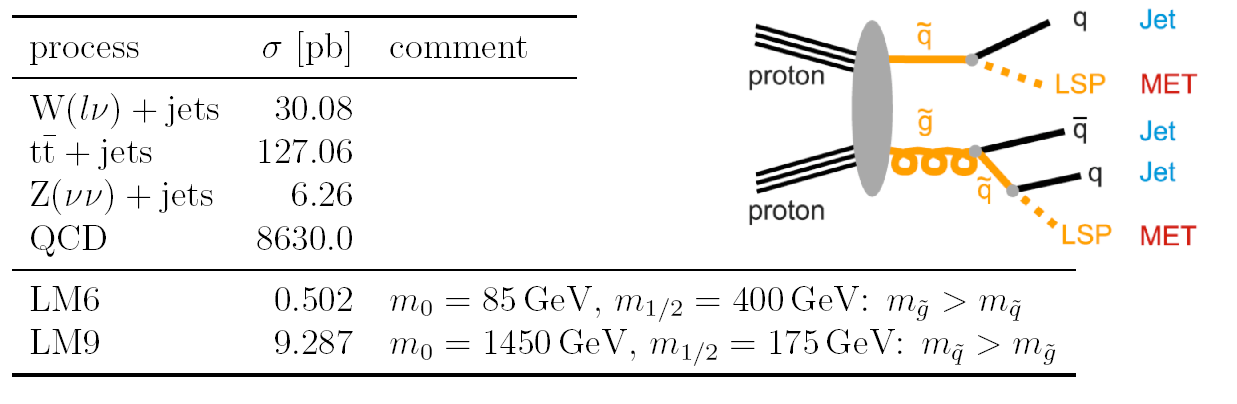
\includegraphics[width=\textwidth,]{figures/feynman+bkg.png}
	\end{figure}
\end{frame}

